\documentclass[border=2pt]{standalone}
\usepackage{tikz}
\usetikzlibrary{quotes,angles}
\usepackage{amsmath}

\begin{document}

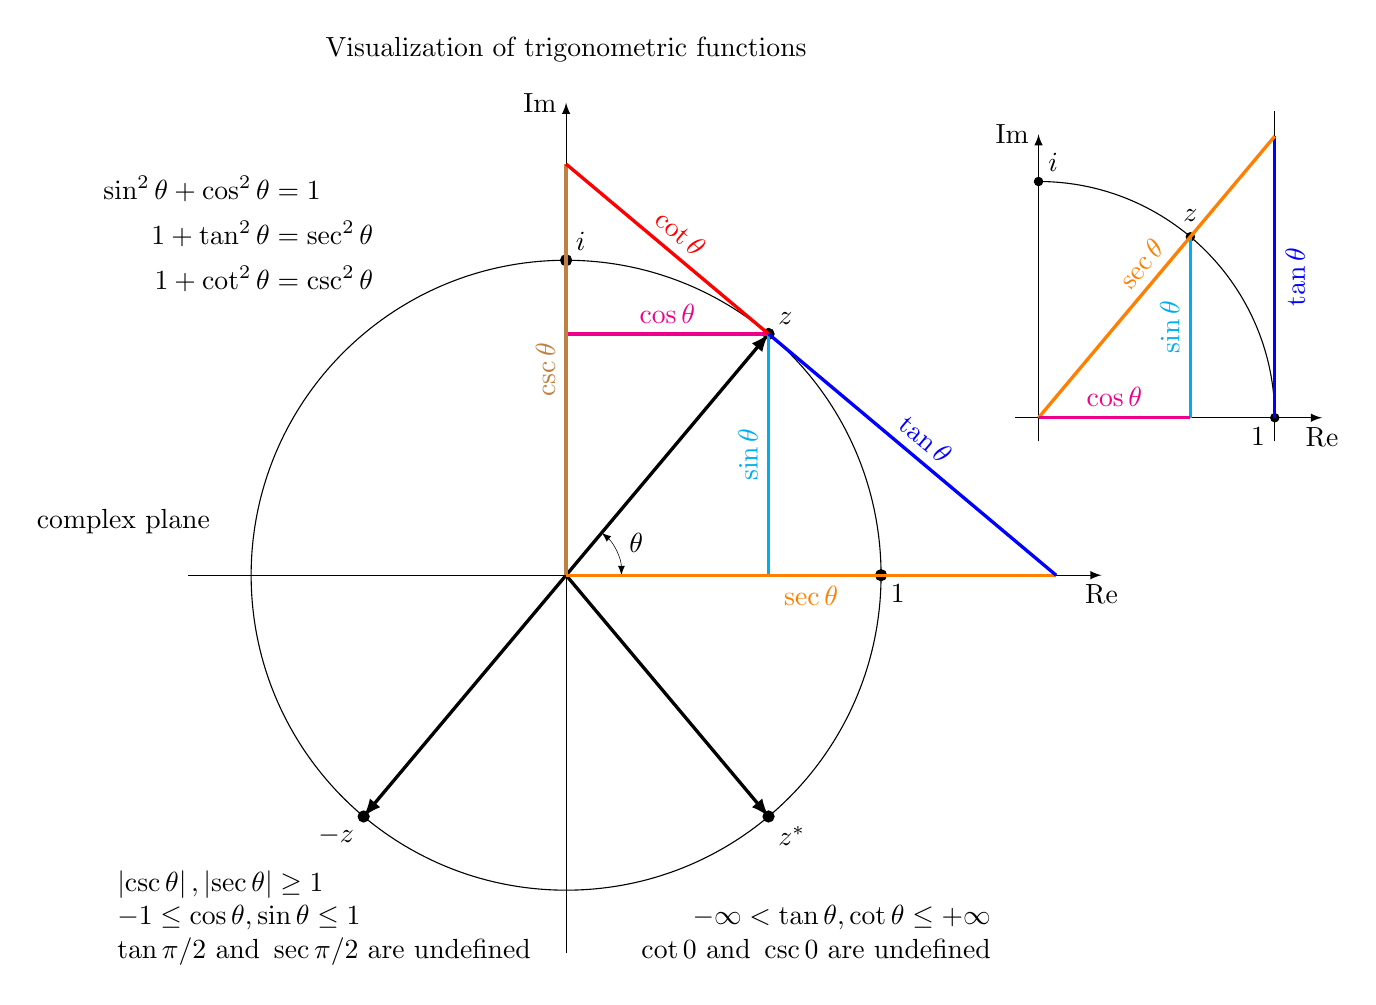
\begin{tikzpicture}[scale=4]

% Draw x and y axis lines
\draw [->,>=latex] (-1.2,0) -- (1.70,0) node [below] {$\mathrm{Re}$};
\draw [->,>=latex] (0,-1.2) -- (0,1.50) node [left ] {$\mathrm{Im}$};
\node[above left] at (-1.1, 0.1) {complex plane};
\filldraw[black] (1,0) circle (0.5pt) node[below right] {$1$} ;
\filldraw[black] (0,1) circle (0.5pt) node[above right] {$i$} ;
\node[above] at (0.0,1.6) {Visualization of trigonometric functions};

% Draw a circle at the origin of radius 1
\draw (0,0) circle (1);

\pgfmathsetmacro{\angle}{50}
\pgfmathsetmacro{\length}{\angle / 180 * pi}


\draw
  (1,0) coordinate (a) 
  -- (0,0) coordinate (b) 
  -- ( {cos(\angle)}, {sin(\angle)} ) coordinate (c) 
  pic["$\theta$", draw=black, very thin, <->,>=latex, angle eccentricity=1.4, angle radius=20]
  {angle=a--b--c};


\draw [very thick,->,>=latex] (0,0) -- ( {cos(\angle)}, {sin(\angle)}) ;
\draw [very thick,->,>=latex] (0,0) -- ( {cos(\angle)},-{sin(\angle)}) ;
\filldraw[black] ( {cos(\angle)}, {sin(\angle)}) circle (0.5pt) node[above right] {$z$} ;
\filldraw[black] ( {cos(\angle)},-{sin(\angle)}) circle (0.5pt) node[below right] {$z^*$} ;
\draw [very thick,->,>=latex] (0,0) -- (-{cos(\angle)},-{sin(\angle)}) ;
\filldraw[black] (-{cos(\angle)},-{sin(\angle)}) circle (0.5pt) node[below left] {$-z$} ;

\draw [very thick, magenta] ( 0, {sin(\angle)}) -- node[above] {$\cos \theta $} ( {cos(\angle)}, {sin(\angle)}) ;
\draw [very thick, cyan] ( {cos(\angle)}, 0) -- node[above, rotate=90] {$\sin \theta $} ( {cos(\angle)}, {sin(\angle)}) ;
\draw [very thick, brown] ( 0, 0) -- node[above, rotate=90] {$\csc \theta $} ( 0, {cosec(\angle)}) ;
\draw [very thick, orange] ( 0, 0) -- node[below] {$\sec \theta $} ( {sec(\angle)}, 0) ;


\begin{scope}[rotate=\angle-90]

\draw [very thick, red] ( {-cot(\angle)}, 1) -- node[above,rotate=\angle-90] {$\cot \theta $} (0,1) ;
\draw [very thick, blue] (0,1) -- node[above,rotate=\angle-90] {$\tan \theta $} ( {tan(\angle)}, 1) ;

\end{scope}

\begin{scope}[shift={( 1.5, 0.5)}, scale=0.75]
\draw [->,>=latex] (-0.1,0) -- (1.2,0) node [below] {$\mathrm{Re}$};
\draw [->,>=latex] (0,-0.1) -- (0,1.2) node [left ] {$\mathrm{Im}$};
\draw (1,0) arc (0:90:1) ;
\filldraw[black] (1,0) circle (0.5pt) node[below left ] {$1$} ;
\filldraw[black] (0,1) circle (0.5pt) node[above right] {$i$} ;
% Draw a line at (1,0)
\draw [very thin] (1,-0.1) -- (1, 1.3)  ;

\filldraw[black] ( {cos(\angle)}, {sin(\angle)}) circle (0.5pt) node[above=2pt ] {$z$} ;
\draw [very thick, blue] (1,0) -- node[below,rotate=90] {$\tan \theta $} (1, {tan(\angle)}) ;
\draw [very thick, cyan] ( {cos(\angle)}, 0) -- node[above, rotate=90] {$\sin \theta $} ( {cos(\angle)}, {sin(\angle)}) ;

%\draw [very thick] (0,0) -- ( 1, {tan(\angle)}) ;
\begin{scope}[rotate=\angle]
\draw [very thick, orange] ( 0, 0) -- node[above, rotate=\angle] {$\sec \theta $} ( {sec(\angle)}, 0) ;
\end{scope}

\draw [very thick, magenta] ( 0, 0) -- node[above] {$\cos \theta $} ( {cos(\angle)}, 0) ;

\end{scope}

\node[below right] at (-1.50, 1.30) {$
\begin{aligned}
\sin^{2}\theta+\cos^{2}\theta & =1\\
1+\tan^{2}\theta & =\sec^{2}\theta\\
1+\cot^{2}\theta & =\csc^{2}\theta
\end{aligned}
$};

\node[below right] at (-1.50, -0.90) {$
\begin{array}{lcr}
\left|\csc\theta\right|,\left|\sec\theta\right|\geq1 & \qquad\\
-1\leq\cos\theta,\sin\theta\leq1 & \qquad & -\infty<\tan\theta,\cot\theta\leq+\infty\\
\tan\pi/2\text{ and }\sec\pi/2\text{ are undefined} & \qquad & \cot0\text{ and }\csc0\text{ are undefined}
\end{array}
$};


\end{tikzpicture}

\end{document}

